\documentclass[12pt, a4paper]{article}
\usepackage[utf8]{inputenc}

\usepackage{hyperref}
\usepackage{float} % To use 'H' for figures
\usepackage{graphicx} % to display images
\usepackage[dvipsnames]{xcolor} % to use colours
\usepackage{amssymb} % For 'mathbb'

\usepackage[normalem]{ulem} % underlying that breaks at line end

\usepackage{amsmath} % for advanced math formatting
\usepackage{amssymb} % for advanced math formatting

\usepackage{titlesec} % Title/Section Styling

\let\stdsection\section
\renewcommand\section{\newpage\stdsection} % Start each section from new page

\titleformat{\section} % uline sections
  {\normalfont\Large\bfseries}{\thesection}{1em}{}[{\titlerule[0.8pt]}]


\setcounter{secnumdepth}{5}
\setcounter{tocdepth}{5}
\makeatletter
\newcommand\subsubsubsection{\@startsection{paragraph}{4}{\z@}{-2.5ex\@plus -1ex \@minus -.25ex}{1.25ex \@plus .25ex}{\normalfont\normalsize\bfseries}}
\newcommand\subsubsubsubsection{\@startsection{subparagraph}{5}{\z@}{-2.5ex\@plus -1ex \@minus -.25ex}{1.25ex \@plus .25ex}{\normalfont\normalsize\bfseries}}
\makeatother

\setlength{\parindent}{0em}
\setlength{\parskip}{1em}

\title{Machine Learning: Supervised Methods
NOTES}
\author{Kristian Bonnici}


\begin{document}



\maketitle
\tableofcontents

\begin{abstract}
These notes cover some of the key concepts in supervised learning. However it's not intended to be a comprehensive introduction into supervised methods. To get most out of the notes, one should have some base knowledge on machine learning and basic algebra.
\end{abstract}

\newpage
\part{Theory}
\newpage

\section{Introduction}

\subsection{Theoretical paradigms }\label{theoretical-paradigms}

Theoretical paradigms for machine learning \textbf{differ} mainly on
what they \uline{assume about the process generating the data}:

\begin{figure}[H]
  \centering  % Remember to centre the figure
    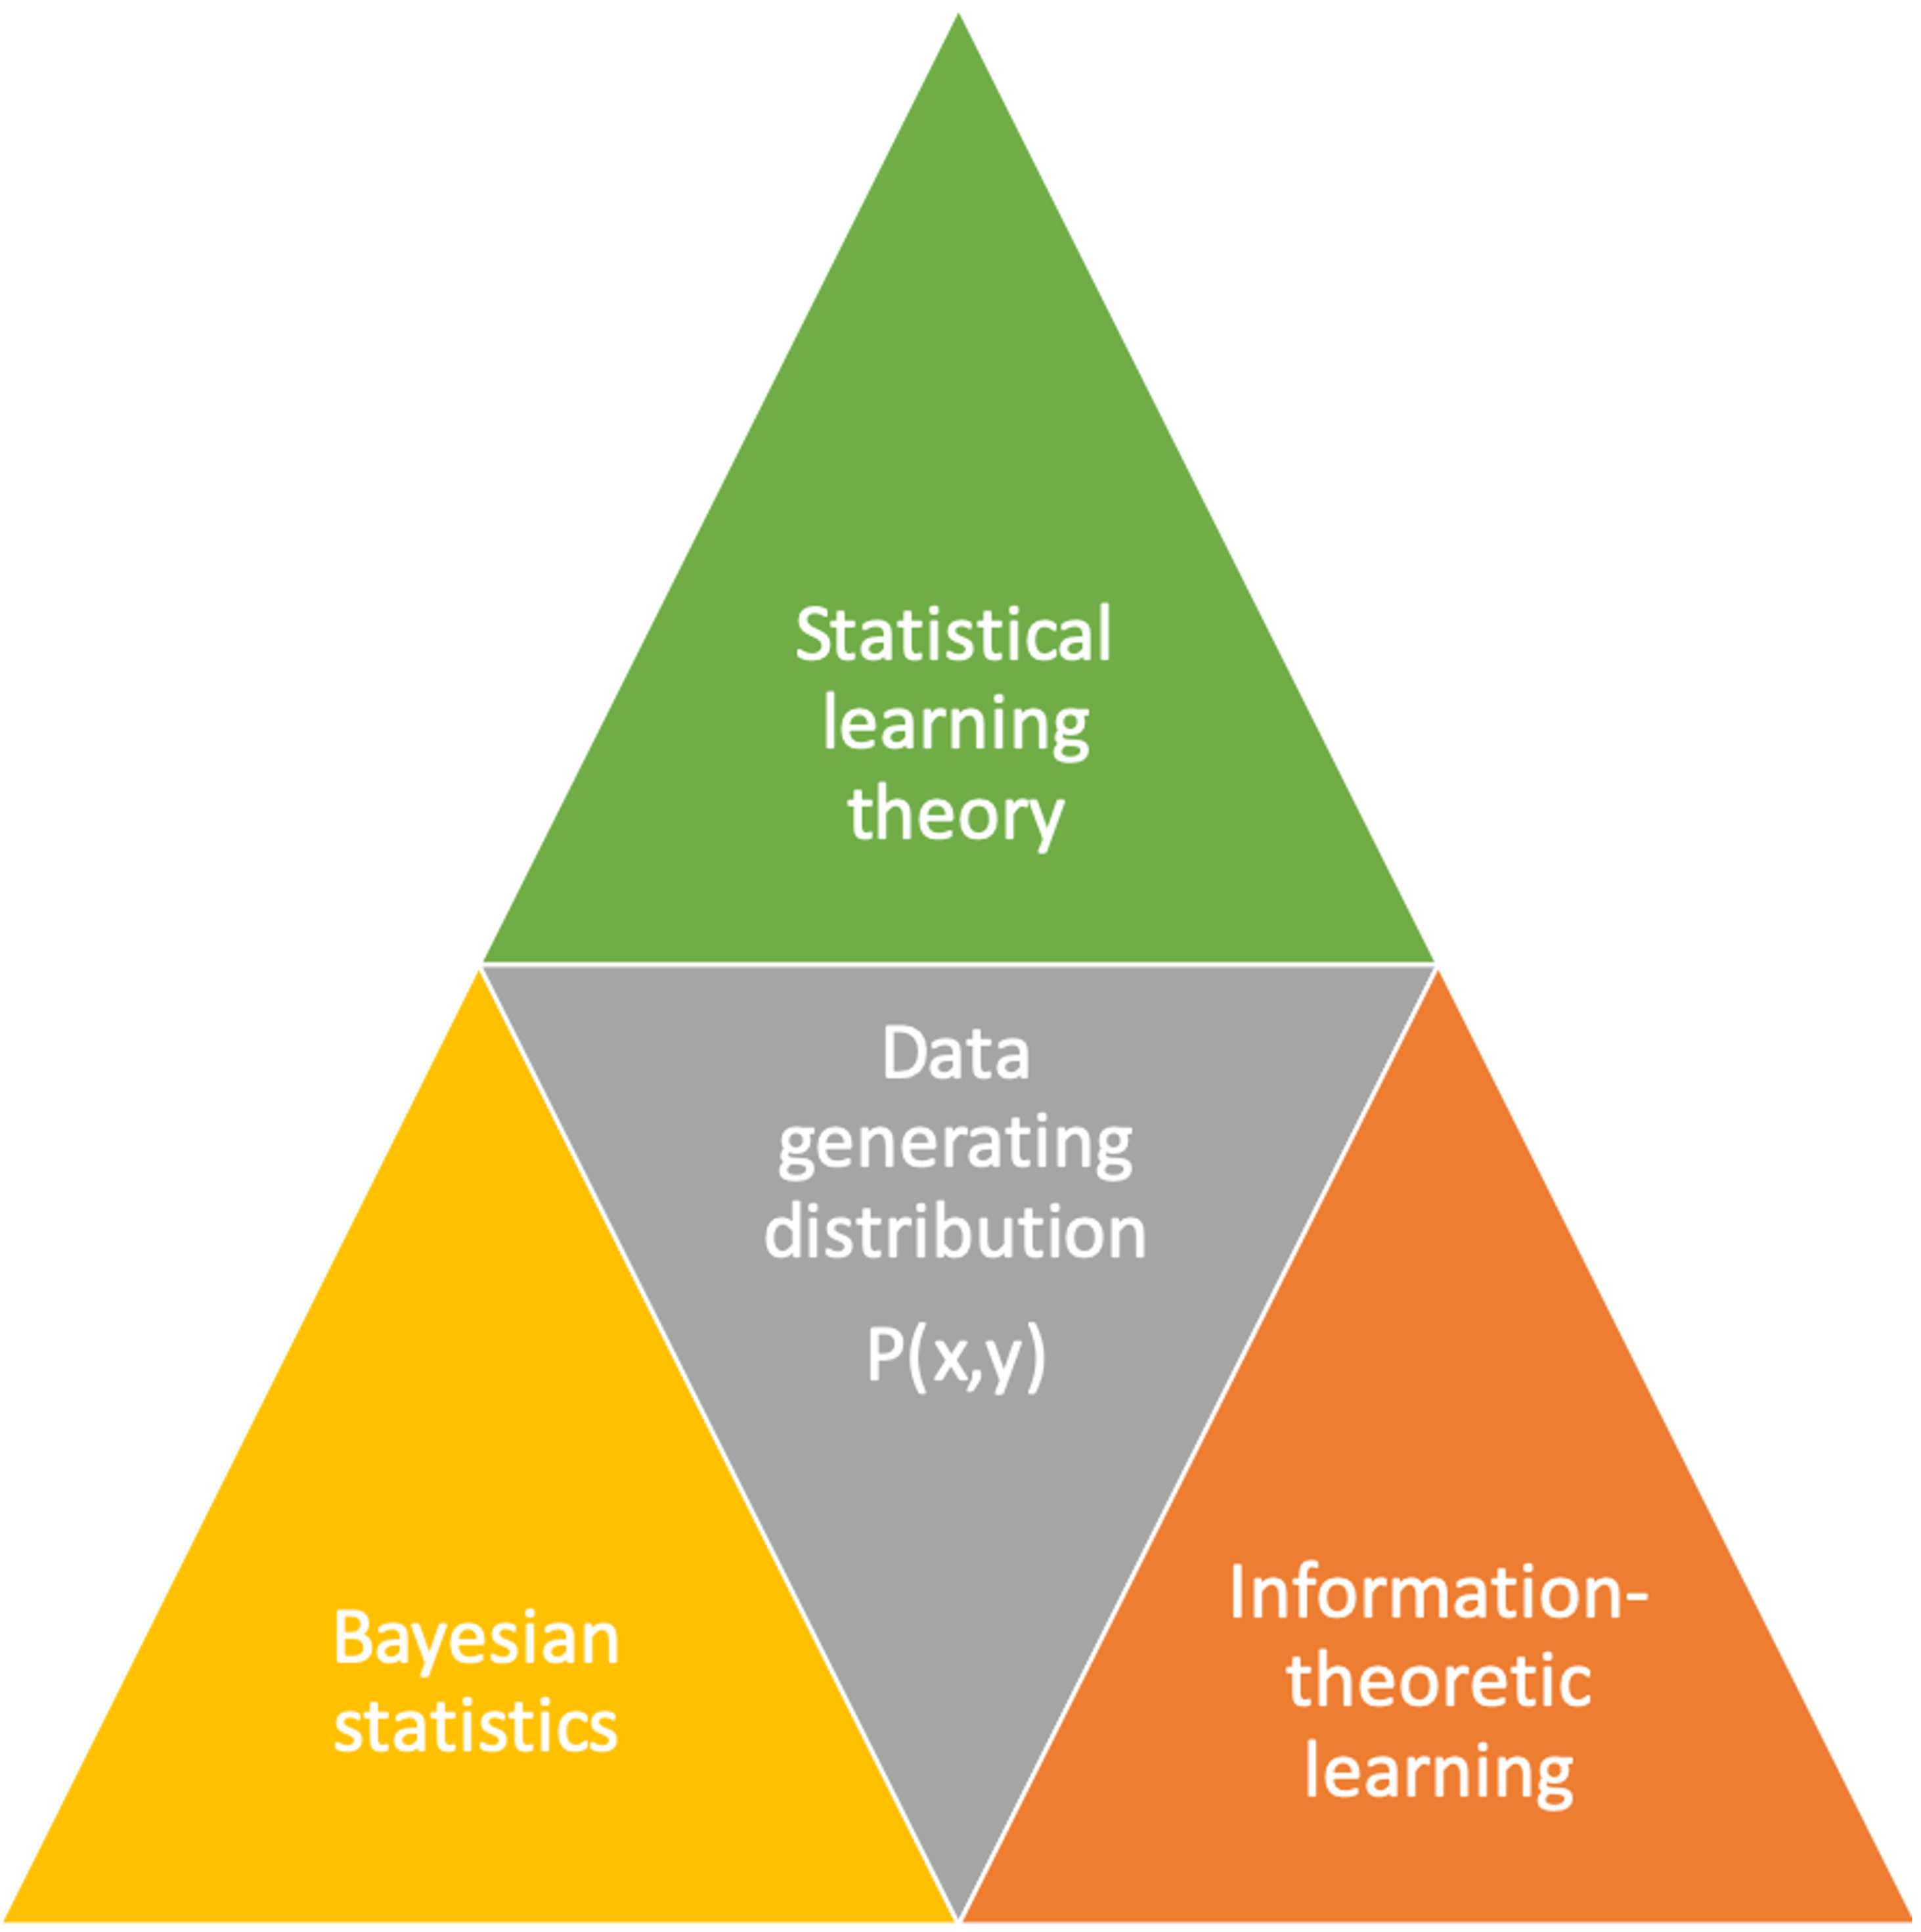
\includegraphics[width=0.4\columnwidth]{images/theoretical-paradigms.png}
    \caption{Paradigms for data generation distributions}
    \label{fig:fig1}
\end{figure}

\begin{itemize}
\item
  \textbf{\textcolor[HTML]{7EAA55}{Statistical learning theory (focus on this course)}:} assumes
  data is \uline{i.i.d} from an \uline{unknown distribution P(x)}, does not estimate the
  distribution (directly)
\item
  \textbf{\textcolor[HTML]{F5C342}{Bayesian Statistics}:} assumes \uline{prior information on P(x)}, estimates posterior probabilities
\item
  \textbf{\textcolor[HTML]{DE8344}{Information theoretic learning}:} (e.g.Minimum Description Length principle, MDL):
  estimates distributions, but does not assume a prior on P(x)

\end{itemize}

\subsection{Dimensions of a supervised learning algorithm
}\label{dimensions-of-a-supervised-learning-algorithm}

\begin{enumerate}
\def\labelenumi{\arabic{enumi}.}
\item
  \textbf{Training sample:} $S = \{(x_i, y_i)\}^m_{i=1}$ the training
  examples $(x, y) \in X \times Y$ independently drawn from a identical
  distribution $(i.i.d) D$ defined on $X \times Y, X$ is a space of inputs,
  $Y$ is the space of outputs.
\item
  \textbf{Model or hypothesis:} $h : X \rightarrow Y$ that we use to predict
  outputs given the inputs $x$.
\item
  \textbf{Loss function:} $L : Y \times Y \rightarrow \mathbb{R}, L(...) \geq 0, L(y, y')$ is the
  loss incurred when predicting $y'$ when $y$ is true.
\item
  \textbf{Optimization} procedure to find the hypothesis $h$ that
  minimize the loss on the training sample.
\end{enumerate}



\subsection{Classification (Task 1/3)}

\textbf{Problem:} partitioning the data into pre-defined classes by a
\emph{decision boundary} or \emph{decision surface}.

\textbf{Multi-class classification:} more than two classes

\begin{itemize}
  \item \textbf{Multi-label Classification:} An example can belong to multiple classes at the same time
  \item \textbf{Extreme classification:} Learning with thousands to hundreds of thousands of classes (Prof.~Rohit Babbar @ Aalto)
\end{itemize}



\subsubsection{Version space}\label{version-space}

\textbf{Version space:} the set of \uline{all \textcolor{blue}{consistent hypotheses}} of the
hypothesis class

\begin{itemize}
  \item
    \textbf{\textcolor{blue}{Consistent hypothesis}:} if correctly classifies all training
    examples
  \item
    \textbf{In version space:}
  \begin{itemize}
    \item
      \textbf{Most general hypothesis $G$:} cannot be expanded without
      including negative training examples
    \item
      \textbf{Most specific hypothesis $S$:} cannot be made smaller
      without excluding positive training points
  \end{itemize}
\end{itemize}

\begin{figure}[H]
  \centering  % Remember to centre the figure
    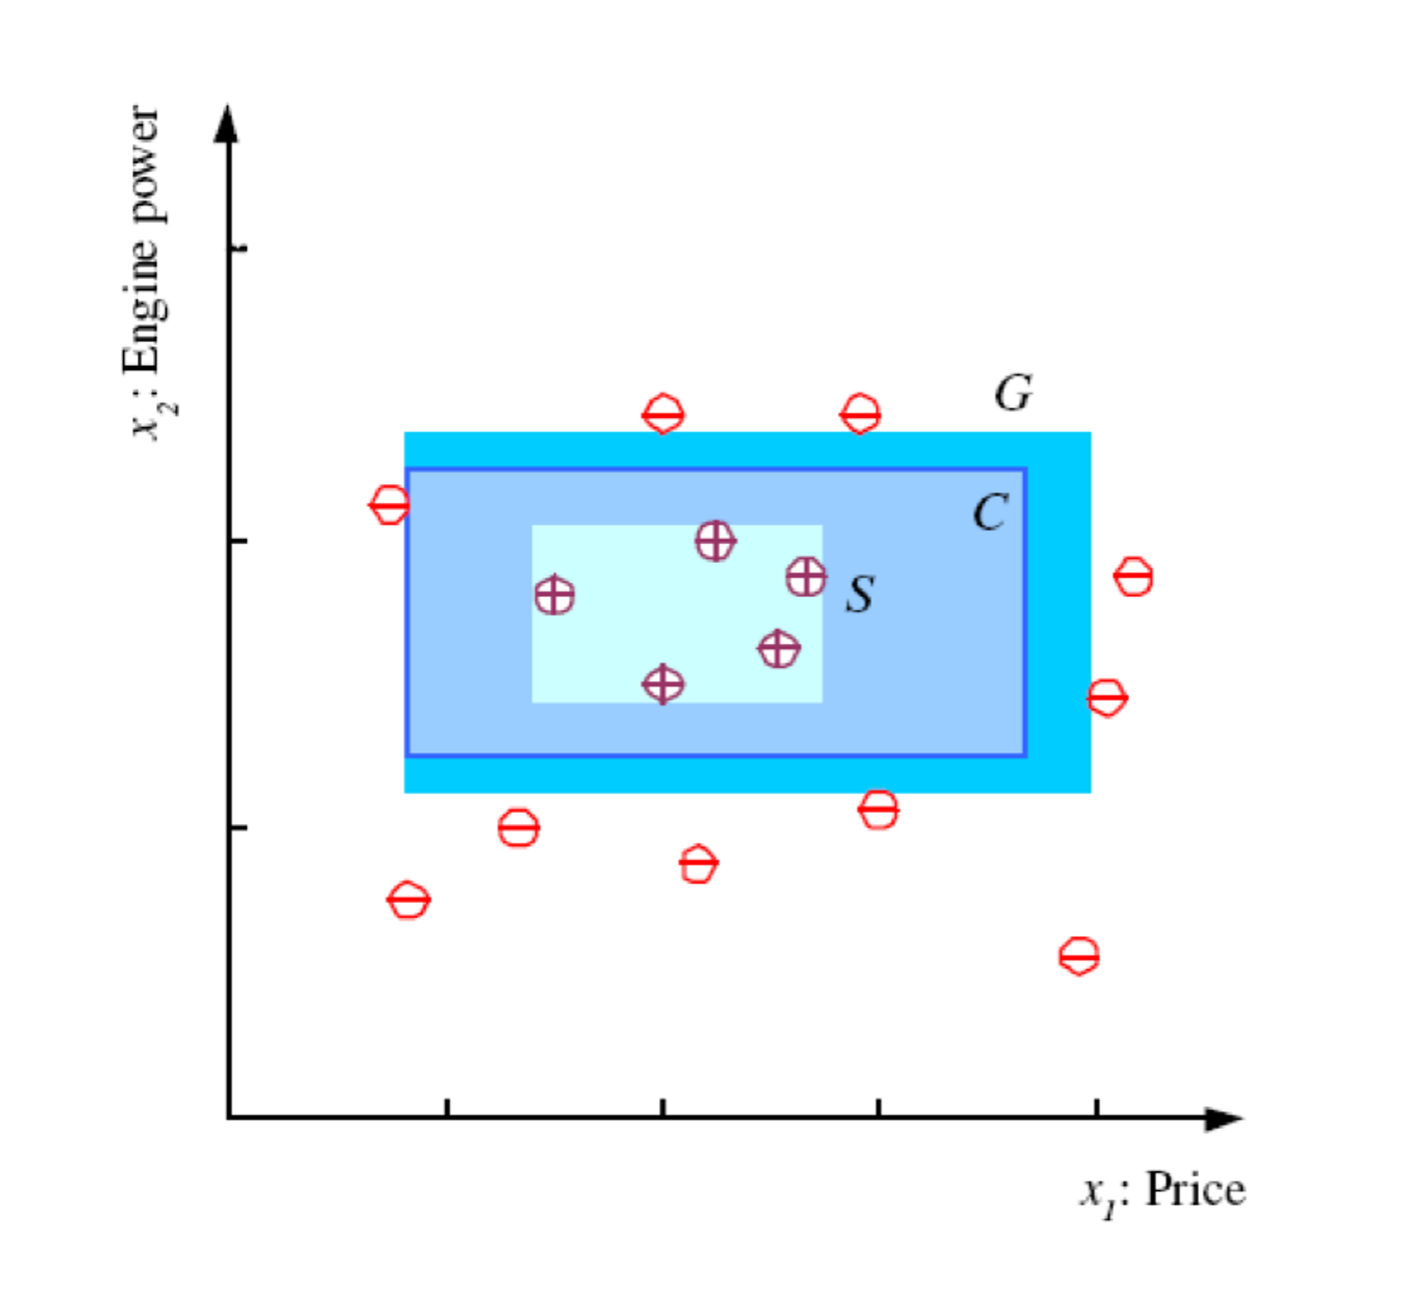
\includegraphics[width=0.5\columnwidth]{images/version-space.png}
    \caption{Illustration of a Version Space.}
    \label{fig:fig2}
\end{figure}

\begin{itemize}
\itemsep1pt\parskip0pt\parsep0pt
\item
  Intuitively, the \textbf{''safest'' hypothesis} to choose from the
  version space is the one that is furthers from the positive and
  negative training examples $\rightarrow$ maximum margin

  \begin{itemize}
  \itemsep1pt\parskip0pt\parsep0pt
  \item
    Margin = minimum distance between the decision boundary and a
    training point
  \end{itemize}
\end{itemize}






\subsection{Regression (Task 2/3) }\label{regression}

\textbf{Problem:} output variables which are numeric.





\subsection{Ranking \& preference learning (Task 3/3)
}\label{ranking-preference-learning}

\textbf{Problem:} predict a ordered list of preferred objects.

\textbf{Training data (typically):} pairwise preferences.

\begin{itemize}
  \item e.g.~user $x$ prefers movie $y_i$ over movie $y_j$
\end{itemize}

\textbf{Output:} ranked list of elements.




\subsection{Generalization}\label{generalization}

\textbf{Aim:} predict as well as possible the outputs of future
examples, not only for training sample.

We would like to \emph{minimize} the \textbf{generalization error}, or
the \textbf{(true) risk}:

\begin{equation} \label{eq:1}
  R(h) = E_{(x,y) \sim D}[L(h(x), y)]
\end{equation}
\begin{gather*}
  \textbf{Where:} \\
  \textbf{D}: \text{\uline{Unknown} distribution where from training and future} \\ \text{examples are drawn from (\uline{i.i.d assumption})}
\end{gather*}

\textbf{What can we say about $R(h)$} based on training examples and the
hypothesis class $\mathcal{H}$ alone? \uline{Two possibilities}:

\begin{itemize}
  \item Empirical evaluation by testing (Section \ref{model-evaluation-by-testing})
  \item Statistical learning theory (Section \ref{statistical-learning-theory})
\end{itemize}






\subsubsection{Model evaluation by testing
}\label{model-evaluation-by-testing}

\textbf{What:} estimate the model's ability to generalize on future data

\textbf{How:} approximating true risk by computing the
empirical risk on a independent test sample:

\[R_{test}(h) = \sum_{(x_i,y_i) \in S_{test}}^{m} L(h(x_i),y_i)\]

\begin{itemize}
  \item The expectation of $R_{test}(h)$ is the true risk $R(h)$
\end{itemize}




\subsection{Hypothesis classes }\label{hypothesis-classes}

There is a huge number of different \textbf{\textcolor{blue}{hypothesis classes}} or
\textbf{\textcolor{blue}{model families}} in machine learning, \textbf{e.g:}

\begin{itemize}
  \item
    \textbf{Linear models} such as logistic regression and perceptron
  \item
    \textbf{Neural networks:} compute non-linear input-output mappings
    through a network of simple computation units
  \item
    \textbf{Kernel methods:} implicitly compute non-linear mappings into
    high-dimensional feature spaces (e.g.~SVMs)
  \item
    \textbf{Ensemble methods:} combine simpler models into powerful
    combined models (e.g.~Random Forests)
\end{itemize}

Each have their different pros and cons in different dimensions
(accuracy, efficiency, interpretability); No single best hypothesis
class exists that would be superior to all others in all circumstances

\begin{center}\rule{3in}{0.4pt}\end{center}






\section{Statistical Learning Theory
}\label{statistical-learning-theory}

\textbf{What:} Statistical learning theory focuses in analyzing the generalization ability of learning algorithms. It's the theoretical background on machine learning.

\textbf{Goal:} Generalization (Section \ref{generalization})






\subsection{Probably Approximately Correct (PAC) learning
}\label{probably-approximately-correct-pac-learning}

\textbf{What:} The most studied \emph{theoretical framework} for \uline{analyzing the generalization performance} of machine learning algorithms. It formalizes the notion of generalization in machine learning. In practice, it's asking for bounding the generaliation error $(\epsilon)$ with high probability $(1 - \delta)$, with arbitrary level of error $\epsilon > 0$ and confidence $\delta > 0$.

\textbf{Ingredients:}

\begin{itemize}
  \item
    \textbf{input space $X$} containing all possible \textbf{inputs $x$}
  \item
    set of possible \textbf{labels $Y$} $($in binary
    classification $Y = \{0, 1\}$$)$
  \item
    \textbf{concept class $\mathcal{C}$} contains \textbf{concepts $C : X \rightarrow Y$} (to be learned),
    concept $C$ gives a label $C(x)$ for each input $x$
    \begin{itemize}
      \item \textcolor{Green}{underlying ground truth} $\rightarrow$ to be learn in the ideal case
      \item \textcolor{Red}{unknown in practice} (or otherwise ML is not needed)
    \end{itemize}
  \item Unknown (i.i.d) \textbf{probability distribution $D$} for the data
  \item \textbf{training sample $S = (x_1,C(x_1)),...,(x_m,C(x_m))$} drawn independently from $D$
  \item \textbf{hypothesis class $\mathcal{H}$}
  \begin{itemize}
    \item in the \textbf{basic case $\mathcal{H} = \mathcal{C}$} but this \colorbox{Yellow}{assumption can be relaxed}
  \end{itemize}
\end{itemize}

\textbf{Goal:} to learn a \uline{hypothesis with a low generalization error}. For 0/1 loss:

\[R(h) = E_{x \sim D} [L_{0/1}(h(x), C(x))] = Pr_{x \sim D} (h(x) \neq C(x))\]





\subsubsection{PAC learnability
}\label{pac-learnability}

\textbf{What:} Question, can we learn a concept class.

\bigskip \bigskip

\textbf{\textcolor{Green}{PAC-learnable}} concept class $\mathcal{C}$ if:

\begin{itemize}
  \item
     \uline{if there exist} an \textbf{algorithm $\mathcal{A}$} that given a training sample $S$ outputs a hypothesis $h_S \in \mathcal{H}$ that has generalization error satisfying
\end{itemize}

\begin{equation} \label{eq:2}
  Pr(\underbrace{R(\overbrace{h_S}^\text{chosen hypothesis from $\mathcal{H}$}) \leq \epsilon}_\text{"low generalization error" event}) \geq \underbrace{1 - \delta}_\text{success rate}
\end{equation}
\begin{gather*}
  P(GeneralizationError\;of\;h_S \leq GeneralizationError\;of\;interest) \geq Desired\;SuccessRate \\
  P(selection\;hypothesis\;(from \; \mathcal{H})\;with\;GeneralizationError \leq \epsilon) \geq Desired\;SuccessRate \\
  Probability\;of\;low\;GeneralizationError \geq Desired\;SuccessRate \\ \\
  \textbf{Where:} \\
  \textbf{$h_S$: } \text{output hypothesis} \\
  \textbf{$S$: } \text{training sample} \\
  \textbf{$m = |S|$: } \text{sample size that grows polynomially in $1/\epsilon$, $1/\delta$} \\
  \textbf{$\epsilon$: } \text{generalization error of interest (arbitrary)} \\
  \textbf{$1-\delta$: } \text{desired success rate / confidence (arbitrary)} \\
\end{gather*}


\textbf{\textcolor{Green}{Efficiently PAC-learnable}} concept class $\mathcal{C}$ if:

\begin{itemize}
  \item
     \textbf{\textcolor{Green}{PAC-learnable}}
   \item
      $\mathcal{A}$ runs in time polynomial in $m$, $1/\epsilon$, and $1/\delta$
      \begin{itemize}
        \item We want the \uline{requirement for training data} and \uline{running time} \textbf{not to explode} when we make $\epsilon$ and $\delta$ stricter $\rightarrow$ requirement of polynomial growth
      \end{itemize}
\end{itemize}


\textbf{Interpretation:}
\begin{itemize}
  \item $\epsilon$: sets the \uline{level of generalization error that is of interest} to us
  \begin{itemize}
    \item e.g. say we are satisfied with \textcolor{Red}{predicting incorrectly $10\%$} of the new datapoints $\rightarrow \epsilon = 0.10$
  \end{itemize}
  \item $1-\delta$: sets a \uline{level of confidence that is of interest} to us
  \begin{itemize}
    \item e.g. say we are satisfied of the \textcolor{Red}{training algorithm to fail $5\%$ of the time to provide a good hypothesis} $\rightarrow \delta = 0.05$
  \end{itemize}
  \item $\{R(h_S ) \leq \epsilon\}$: The \uline{event ”low generalization error”}
  \begin{itemize}
    \item considered as a \textit{random variable} because we cannot know beforehand which hypothesis $h_S \in \mathcal{H}$ will be selected by the algorithm
  \end{itemize}
\end{itemize}

\begin{figure}[H]
  \centering  % Remember to centre the figure
    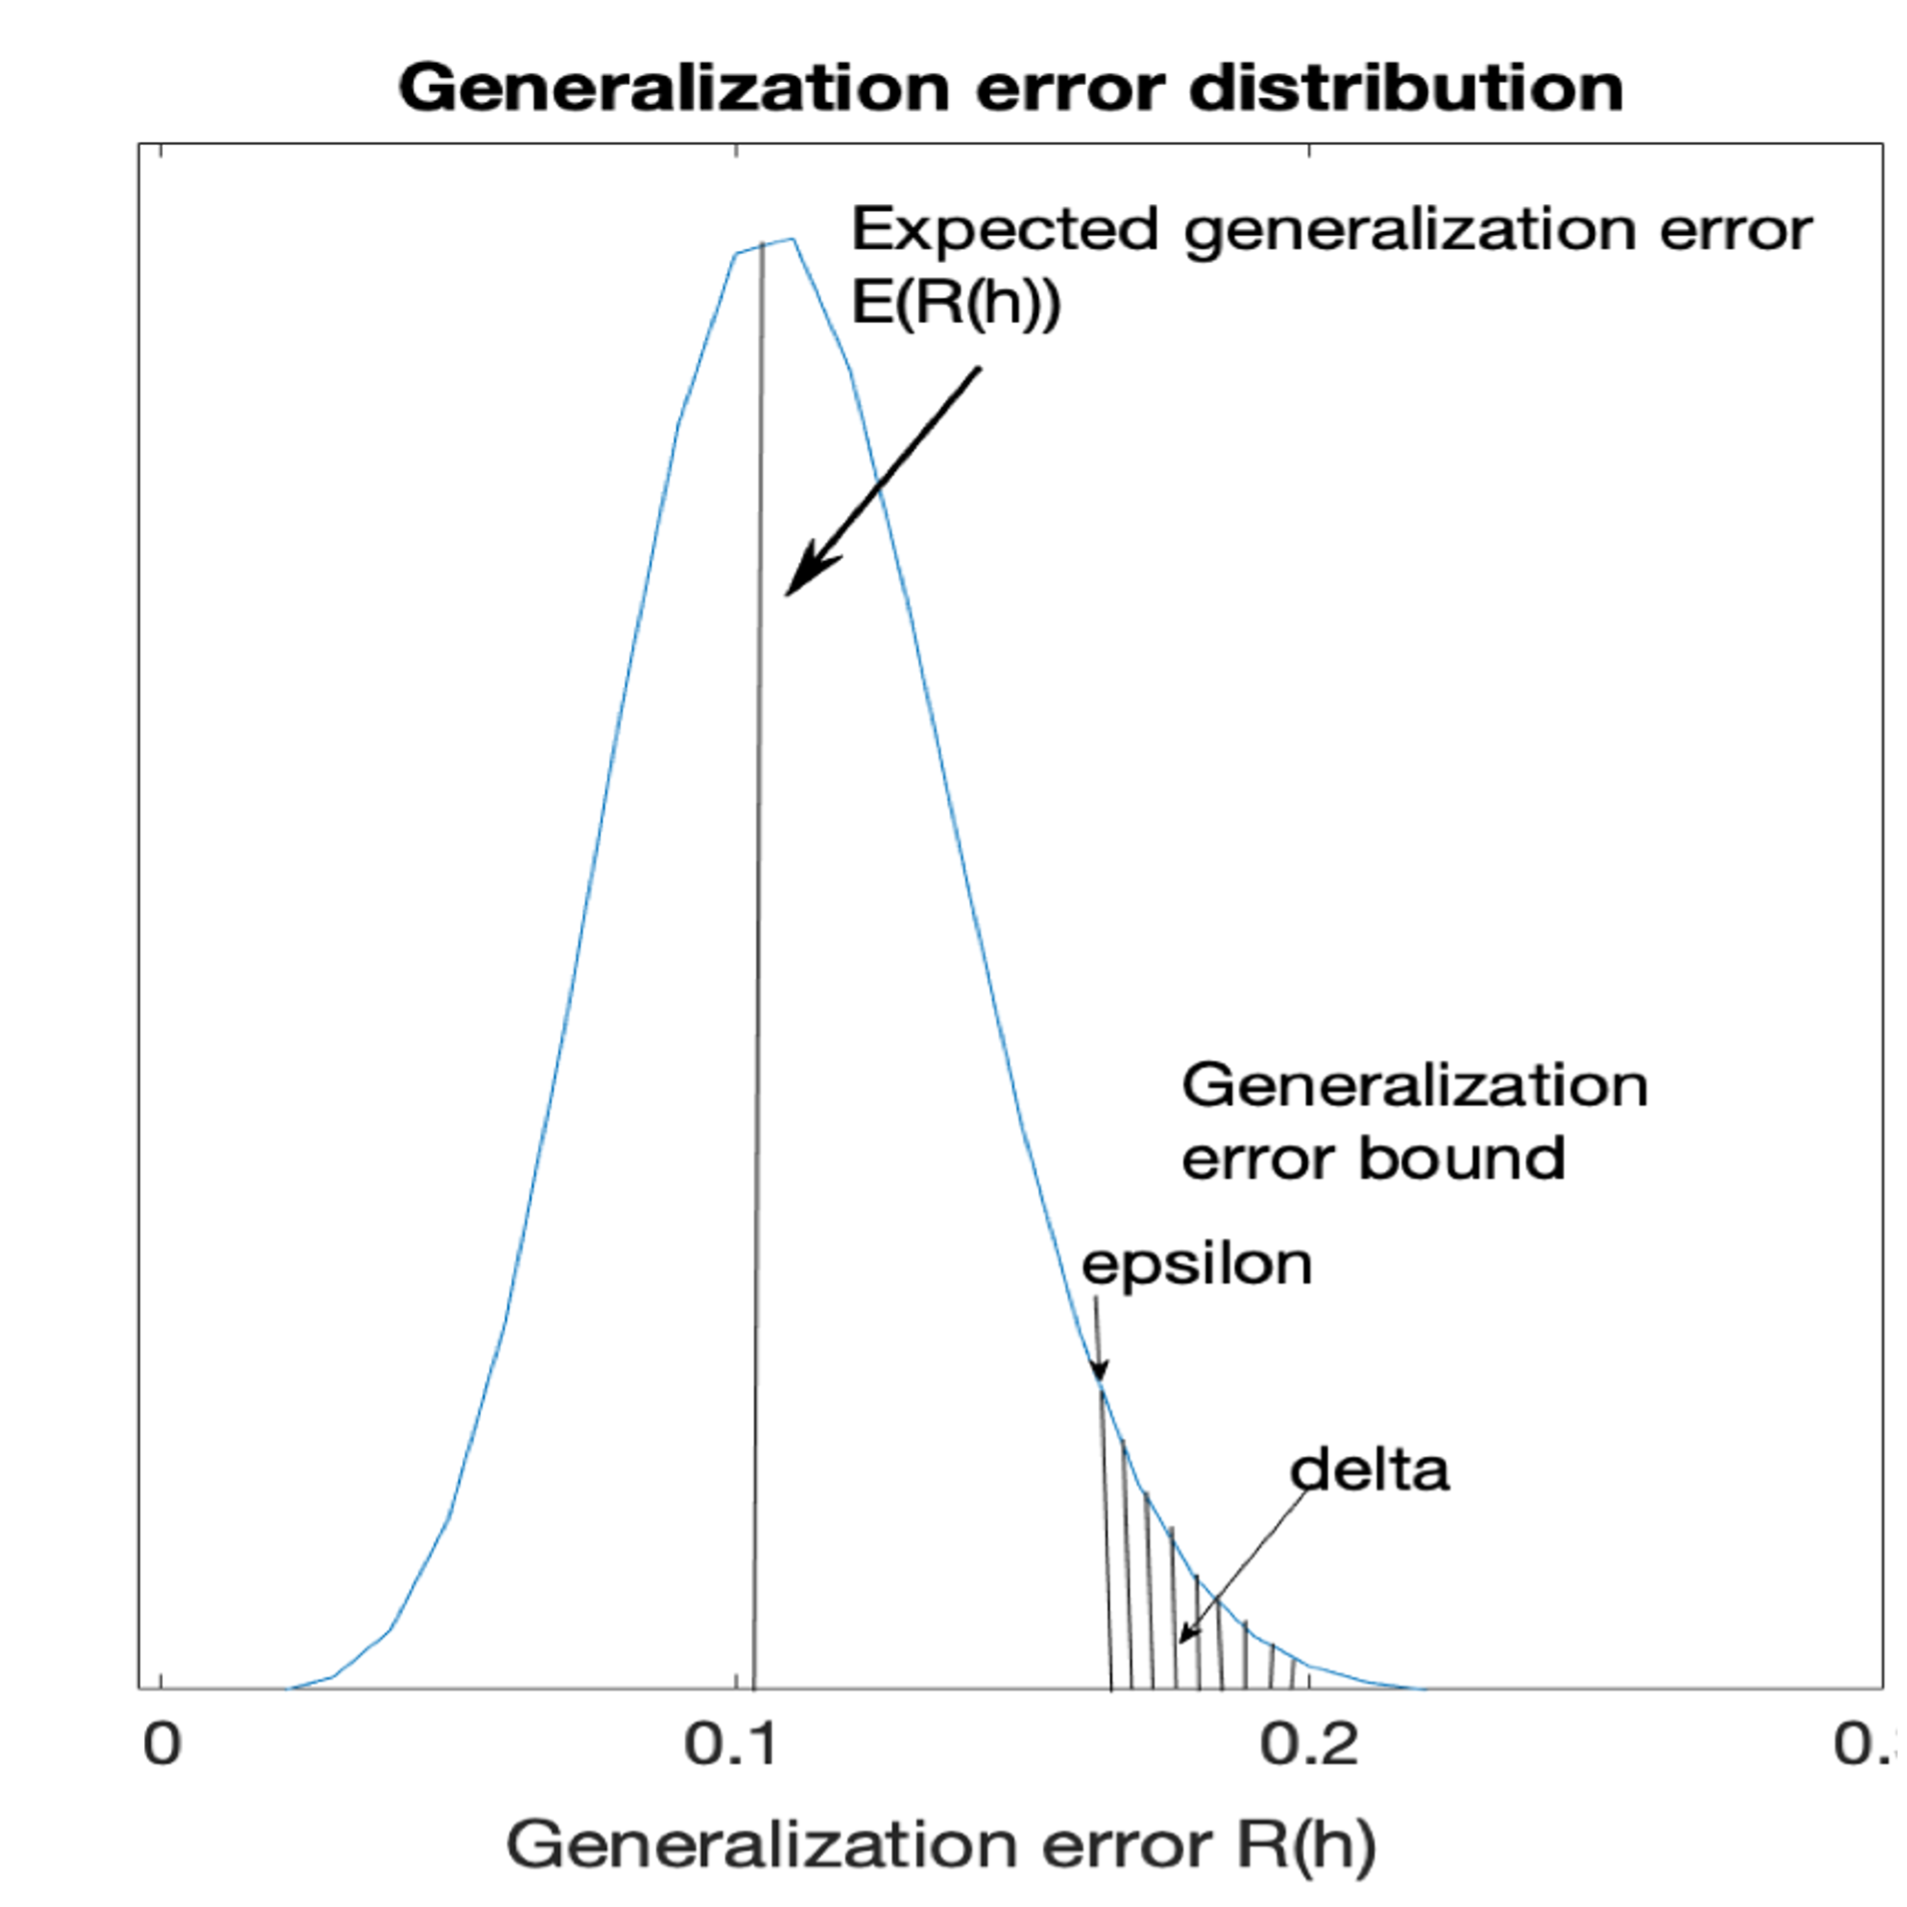
\includegraphics[width=0.6\columnwidth]{images/generalization-error-distribution.png}
    \caption{Generalization error distribution and error bound}
    \label{fig:fig3}
\end{figure}


\textbf{Generalization error bound vs. expected test error:}

\begin{itemize}
  \item We \uline{bound the probability of being in the high error tail} of the distribution (\uline{not the convergence to the mean or median generalization error}) $\rightarrow$ thus \textbf{empirically estimated test errors} might be considerably \uline{lower than the bounds suggest}.
\end{itemize}





\subsection{Learning with finite hypothesis classes
}\label{learning-with-finite-hypothesis-classes}

\textbf{What:} Finite concept classes arise when:

\begin{itemize}
  \item \textbf{Input variables} \uline{have finite domains} or they are converted to such in preprocessing (e.g. discretizing real values)
  \item The \uline{representations of the hypotheses have finite size} (e.g. the number of times a single variable can appear)
\end{itemize}

\bigskip \bigskip

\textbf{Finite hypothesis class - consistent case}

\begin{itemize}
  \item \textbf{Sample complexity bound} relying on the size of the hypothesis class (Mohri et al, 2018): $Pr(R(h_S) \leq \epsilon) \geq 1 - \delta$ if
  \[
  m \geq \frac{1}{\epsilon}(log(|\mathcal{H}|) + log(\frac{1}{\delta}))
  \]
  \item An equivalent \textbf{generalization error bound}:
  \[
  R(h) \leq \frac{1}{m}(log(|\mathcal{H}|) + log(\frac{1}{\delta}))
  \]
  \item \textbf{Holds for} \uline{any finite hypothesis class}
  \textbf{assuming there is a} \uline{consistent hypothesis}, \uline{one with zero empirical risk} \colorbox{Yellow}{or close to it (relaxed)}.
  \item The \uline{more hypotheses} there are in $\mathcal{H} \rightarrow$ the \uline{more training examples are needed}
\end{itemize}


\subsubsection{Example: Boolean conjunctions
}\label{example-boolean-conjunctions}


\textbf{What:} Example of a finity hypothesis class.

\bigskip \bigskip


\textbf{Example hypothesis class:} Boolean conjunctions

\begin{itemize}
  \item Dealing with subclasses of Boolean formulae, expressions \textbf{binary input variables} (literals) combined with \textbf{logical operators} \uline{AND} \& \uline{NOT}.
\end{itemize}

\bigskip \bigskip


\textbf{Example case:} Aldo likes to do sport only when the weather is suitable

\begin{itemize}
  \item \textbf{Training data:} Also has given examples of suitable and not suitable weather

  \begin{center}
    \begin{tabular}{ |c|c c c c c c|c| }
     \hline
      & \multicolumn{6}{|c|}{$x^t$} & $r(x^t)$ \\
       t & Sky & AirTemp & Humidity & Wind & Water & Forecast & EnjoySport \\
       \hline
       1 & Sunny & Warm & Normal & Strong & Warm & Same & 1 \\
       2 & Sunny & Warm & High & Strong & Warm & Same & 1 \\
       3 & Rainy & Cold & High & Strong & Warm & Change & 0 \\
       4 & Sunny & Warm & High & Strong & Cool & Change & 1 \\
       \multicolumn{8}{|c|}{} \\
       \multicolumn{8}{|c|}{\textcolor{blue}{Table:} Aldo's observed sport experiences in different weather conditions.} \\
     \hline
    \end{tabular}
  \end{center}

  \item \textbf{Model:} Let us build a classifier (boolean formulae containing AND, and NOT, but not OR operators) for Aldo to decide whether to do sports today
  \begin{itemize}
    \item e.g. if (Sky=Sunny) AND NOT (Wind=Strong) then (EnjoySport=1)
  \end{itemize}

  \item \textbf{Number of hypotheses $|\mathcal{H}|$:}
  \begin{itemize}
    \item \textbf{Each variable:} "AND", "AND NOT", or can be excluded from the rule $\rightarrow$ \uline{3 possibilities}
    \item \textbf{Total number of hypotheses} is thus $3^d$, where d is the number of variables $\rightarrow |\mathcal{H}| = 3^6 = \uline{729}$
  \end{itemize}

  \item \textbf{Plotting the bound for Aldo’s problem using boolean conjunctions:}
  \begin{itemize}
    \item \textbf{Left plot:} generalization bound $\epsilon$ is shown for different values of delta $\delta$, using d = 6 variables.
    \item \textbf{Right plot:} generalization bound $\epsilon$ is shown for increasing number of input variables d, using delta $\delta = 0.05$

    \begin{figure}[H]
      \centering  % Remember to centre the figure
        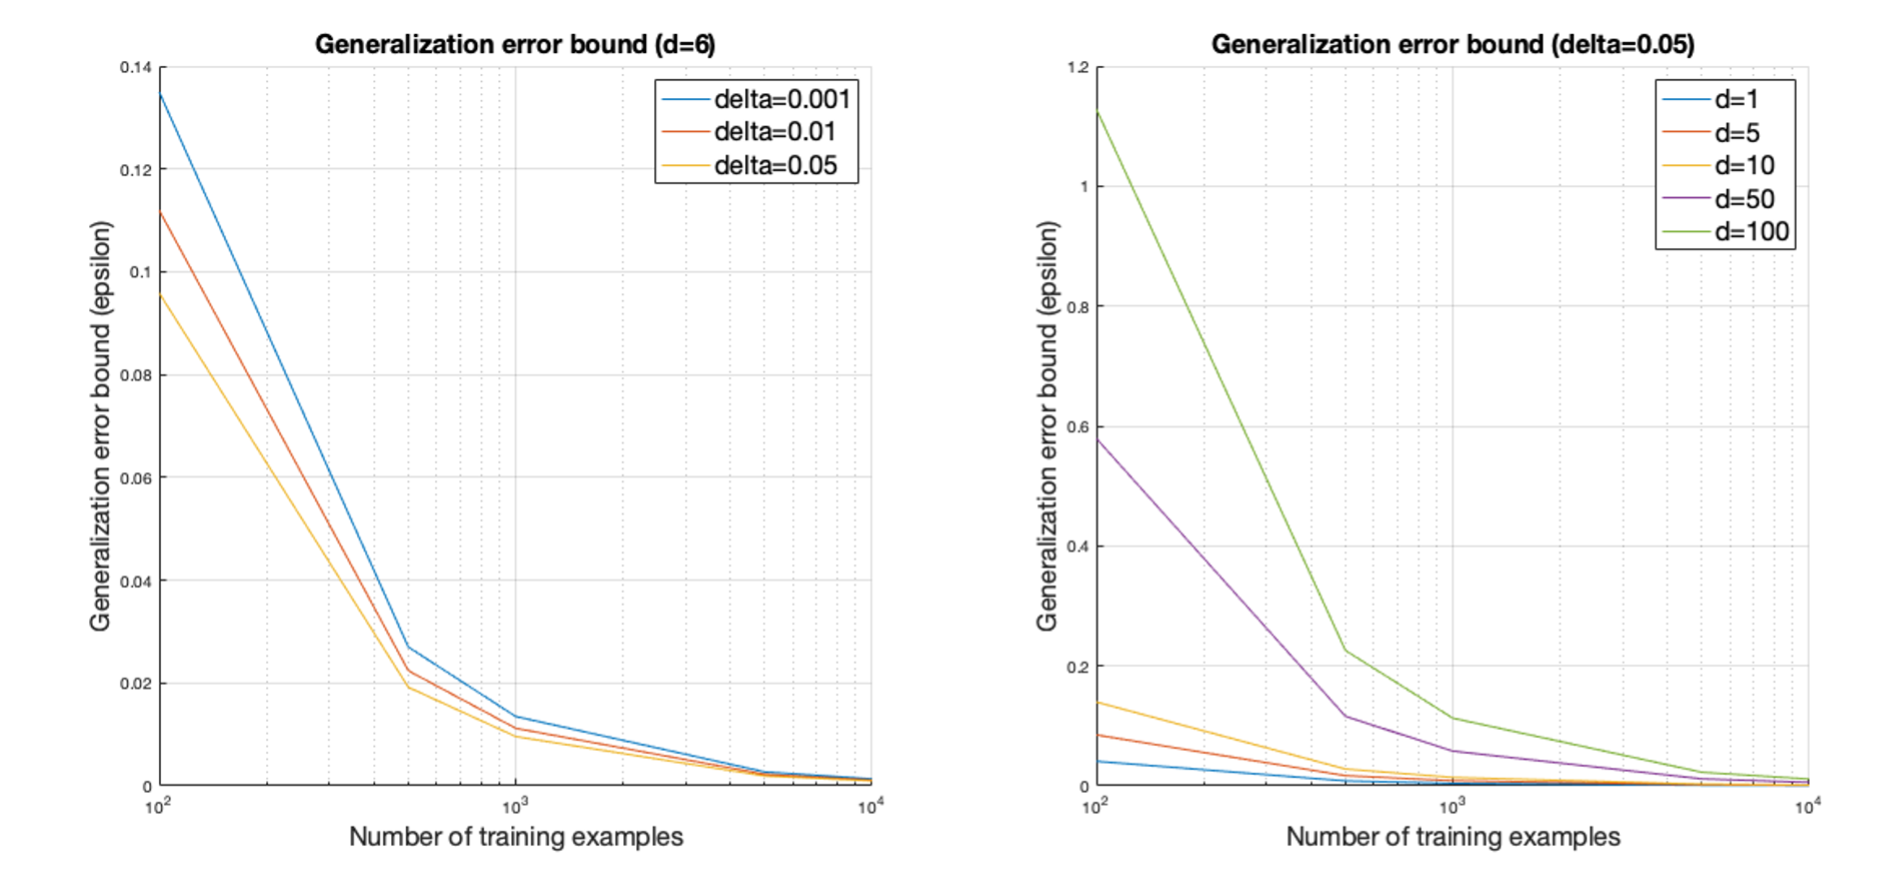
\includegraphics[width=1.0\columnwidth]{images/eg1-generalization-error-bound.png}
        \caption{Boolean conjunctions: Generalization error bounds}
        \label{fig:fig4}
    \end{figure}

  \end{itemize}

  \item \textbf{Typical behaviour of ML learning algorithms is revealed:}
  \begin{itemize}
    \item \textbf{\textcolor{Green}{increase of sample size decreases generalization error}}
    \item extra data gives \textbf{\textcolor{Red}{less and less additional benefit as the sample size grows}} (law of diminishing returns)
    \item requiring high level of confidence (small $\delta$) for obtaining low error requires more data for the same level of error
  \end{itemize}

\end{itemize}






\subsection{Learning with infinite hypothesis classes
}\label{learning-with-infinite-hypothesis-classes}


Most models used in practise rely on infinite hypothesis classes, e.g.

\begin{itemize}
  \item $\mathcal{H}$ = hyperplanes in $\mathbb{R}^d$ (e.g. Support vector machines)
  \item $\mathcal{H}$ = neural networks with continuous input variables
\end{itemize}





\subsubsection{Vapnik-Chervonenkis (VC) dimension}\label{vapnik-chervonenkis-dimension}

\textbf{Purpose:} Vapnik-Chervonenkis dimension lets us \textbf{study} \uline{learnability of infinite hypothesis classes} \textbf{through} the concept of \uline{\textcolor{Purple}{shattering}}

\textbf{What:} can be understood as measuring the \uline{capacity of a hypothesis class to adapt to different concepts}

\begin{itemize}
  \item $VCdim(\mathcal{H}) =$ \uline{size} of the \textbf{largest training set} that we can find a \textbf{consistent classifier for all labelings in $Y^m$}
  \item Intuitively:
  \begin{itemize}
    \item low $VCdim \rightarrow$ easy to learn, low sample complexity
    \item high $VCdim \rightarrow$ hard to learn, high sample complexity
    \item infinite $VCdim \rightarrow$ cannot learn in PAC framework
  \end{itemize}
\end{itemize}

\bigskip \bigskip

\textbf{How to show that $VCdim(\mathcal{H}) = d$ for a hypothesis class:}
\begin{itemize}
  \item We need to show two facts:
  \begin{enumerate}
    \item There \textcolor{Green}{exists} a \uline{set of inputs of size $d$ that \textbf{can be \textcolor{Purple}{shattered}} by hypothesis in $\mathcal{H}$} (i.e. we can pick the set of inputs any way we like): $VCdim(\mathcal{H}) \geq d$
    \item There \textcolor{Red}{does not exist} any \uline{set of inputs of size $d + 1$ that \textbf{can be \textcolor{Purple}{shattered}}} (i.e. need to show a general property): $VCdim(\mathcal{H}) < d + 1$
  \end{enumerate}
\end{itemize}

\bigskip \bigskip

\textbf{Formally:} (for binary labelings)

\begin{itemize}
  \item Through \textbf{growth function}:
    $$
    \sqcap_{\mathcal{H}}(m) = \max_{ \{x_1, ..., x_m\} \subset X } |\{(h(x_1), ..., h(x_m)) : h \in \mathcal{H}\}|
    $$
    \begin{itemize}
      \item The growth function gives the \uline{maximum number of unique labelings} the hypothesis class $\mathcal{H}$ can provide for an arbitrary set of input points
      \item The maximum of the growth function is \uline{$2^m$ for a set of $m$ examples}
    \end{itemize}
    \item \textbf{Vapnik-Chervonenkis dimension} is then
    $$
    VCdim(\mathcal{H}) = \max_{m}\{m | \sqcap_{\mathcal{H}}(m) = 2^m\}
    $$
\end{itemize}





\subsubsubsection{Shattering}\label{shattering}

\textbf{What:} underlying concept in VC dimension

\textbf{Given:} a set of points $S = {x_1,...,x_m}$ and a fixed class of functions $\mathcal{H}$

\textbf{$\mathcal{H}$ is said to \textcolor{Purple}{shatter} $S$ if:} for any possible partition of $S$ into positive $S_+$ and negative subset $S_-$ we can find a hypothesis for which $h(x) = 1$ if and only if $x \in S_+$

\begin{figure}[H]
  \centering  % Remember to centre the figure
    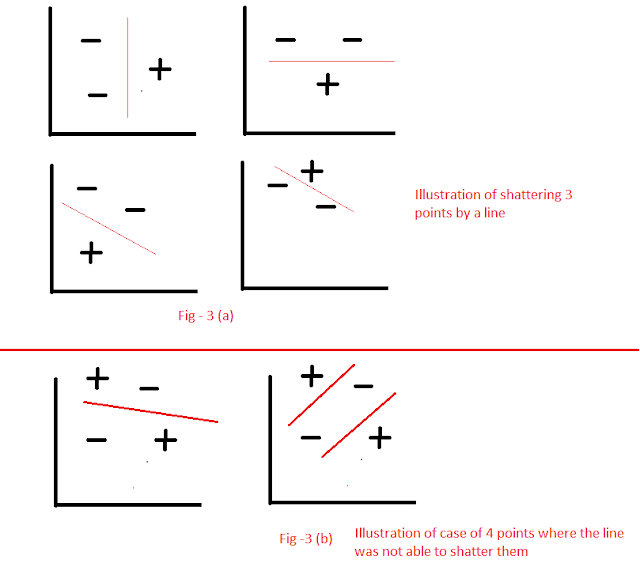
\includegraphics[width=0.9\columnwidth]{images/shattering.png}
    \caption{Illustration of shattering}
    \label{fig:fig5}
\end{figure}





\subsubsubsection{Generalization bound with VC-dimension}\label{deneralization-bound-with-vc-dimension}

\textbf{What:} Way of using VC-dimensions to analyze machine learning algorithms.

(Mohri, 2018) Let $\mathcal{H}$ be a family of functions taking values in ${-1, +1}$ with VC-dimension $d$ . Then for any $\delta > 0$, with probability at least $1 - \delta$ the following holds for all $h \in \mathcal{H}$:

$$
R(h) = \underbrace{\hat{R}(h)}_\text{empirical risk} + \sqrt{\frac{2\log{(em/d)}}{m/d}} + \sqrt{\frac{\log{(1/\delta)}}{2m}}
$$

\begin{gather*}
  \textbf{Where:} \\
  \textbf{$d$: } \text{VC-dimension} \\
  \textbf{$m$: } \text{amount of training data} \\
  \textbf{$e$: } \text{Euler's number, $e \approx 2.71828$} \\
  \textbf{$\delta$: } \text{failure rate} \\
\end{gather*}

\begin{itemize}
  \item $m/d$ shows that changing to a model with higher VC-dimension $d$ makes the same amount of training samples $m$ less effective. $\rightarrow$ the second term grows when VC-dimension grows.
  \begin{itemize}
    \item For more complex $\mathcal{H}$ class, one needs more data $m$ to guarantee similar kind of generalization.
  \end{itemize}
  \item Manifestation of the \textbf{Occam’s razor principle:} to justify an increase in the complexity, we need reciprocally more data
\end{itemize}




\subsubsection{Rademacher complexity}\label{rademacher-complexity}


\textbf{What:} Rademacher complexity defines complexity as the capacity of hypothesis class to fit random noise

\textbf{Why:} Rademacher complexity is a practical alternative to VC dimension, giving typically sharper bounds (but requires a lot of simulations to be run).


\bigskip \bigskip


\textbf{Experiment:} how well does your hypothesis class fit noise?

\begin{itemize}
  \item Consider a \textbf{set of training examples $S_0 = \{(x_i , y_i)\}^m_{i=1}$}
  \item \textbf{Generate $M$ new datasets $S_1 , ... , S_M$} from $S_0$ by randomly drawing a new label $\sigma \in Y$ for each training example in $S_0$
  $$
  S_k = \{(x_i, \sigma_{ik})\}^m_{i=1}
  $$
  \item Train a classifier $h_k$ minimizing the empirical risk on training set $S_k$, record its empirical risk
  $$
  \hat{R}(h_k) = \frac{1}{m} \sum_{i=1}^{m} 1_{h_k(x_i) \neq \sigma_{ik}}
  $$
  \item \textbf{Compute the average empirical risk over all datasets:}
  $$
  \bar{\epsilon} = \frac{1}{M} \sum_{k=1}^{M} \hat{R}(h_k)
  $$
  \item \textbf{Observe the quantity:}
  $$
  \hat{\mathcal{R}} = \frac{1}{2} - \bar{\epsilon}
  $$
  \begin{itemize}
    \item When ($\hat{\mathcal{R}} = 0, \bar{\epsilon} = 0.5$) $\rightarrow$ predictions correspond to random coin flips (0.5 probability to predict either class)
    \item When ($\hat{\mathcal{R}} = 0.5, \bar{\epsilon} = 0$) $\rightarrow$ all hypotheses $h_i , i = 1, ... , M$ have zero empirical error (perfect fit to noise, not good!)
    \item \textbf{Ideally we want:}
    \begin{itemize}
      \item to be able to \textbf{\textcolor{Green}{separate noise from signal}}
      \begin{itemize}
        \item Meaning large $\bar{\epsilon}$, so that the model is bad at classifying random noise. $\rightarrow$ low complexity $\hat{\mathcal{R}}$.
      \end{itemize}
      \item to have \textbf{\textcolor{Green}{low empirical error on real data}} - otherwise impossible to obtain low generalization error
    \end{itemize}
  \end{itemize}
\end{itemize}



\textbf{Rademacher complexity:}

\begin{itemize}
  \item For binary classification with labels $Y = \{-1, +1\}$ \textbf{empirical Rademacher complexity} can be defined as
  $$
  \hat{\mathcal{R}}_S(\mathcal{H}) = \frac{1}{2} E_\sigma (\underbrace{\sup_{h \in \mathcal{H}} \frac{1}{m} \sum_{t=1}^m \overbrace{\sigma^i}^\text{random true label } \overbrace{h(x_i)}^\text{ predicted random label}}_\text{hypothesis with highest correlation with random label})
  $$
  \begin{gather*}
    \textbf{Where:} \\
    \textbf{$\sigma_i \in \{-1, +1\}$: } \text{are Rademacher random variables,} \\
    \text{drawn independently from uniform distribution}  \\
    \text{(i.e. $Pr\{\sigma = 1\} = 0.5)$} \\
  \end{gather*}
  \item We can also rewrite \textbf{$\hat{\mathcal{R}}_S$ in terms of empirical error}
  $$
  \hat{\mathcal{R}}_S = \frac{1}{2} - E_\sigma \inf_{h \in \mathcal{H}} \hat{\epsilon}(h)
  $$
  \begin{itemize}
    \item Now we have Rademacher complexity in terms of \uline{expected minimum error of classifying randomly labeled data}
  \end{itemize}
\end{itemize}





\subsubsubsection{Generalization bound with Rademacher complexity}\label{deneralization-bound-with-rademacher-complexity}

(Mohri et al. 2018): For any $\delta > 0$, with probability at least $1 - \delta$ over a sample drawn from an unknown distribution $D$, for any $h \in \mathcal{H}$ we have:

$$
R(h) \leq \underbrace{\hat{R}_S(h)}_\text{empirical risk} + \underbrace{\hat{\mathcal{R}}_S(\mathcal{H})}_\text{empirical Rademacher complexity} + 3 \sqrt{\frac{\log{\frac{2}{\delta}}}{2m}}
$$





\subsubsection{Vapnik-Chervonenkis dimension VS. Rademacher complexity}\label{vapnik-chervonenkis-dimension-vs-rademacher-complexity}

Note the differences between Rademacher complexity and VC dimension

\begin{itemize}
  \item Dependency on training data
  \begin{itemize}
    \item \textbf{VC dimension:} \uline{independent} $\rightarrow$ measures the \textcolor{Red}{worst-case} where the data is generated in a bad way for the learner
    \item \textbf{Rademacher complexity:} \uline{depends on the training sample} thus is dependent on the data generating distribution
  \end{itemize}
  \item Focus
  \begin{itemize}
    \item \textbf{VC dimension:} extreme case of realizing all labelings of the data
    \item \textbf{Rademacher complexity:} measures smoothly the ability to realize random labelings
  \end{itemize}
\end{itemize}


\bigskip \bigskip


Example: Rademacher and VC bounds on a real dataset


\begin{figure}[H]
  \centering  % Remember to centre the figure
    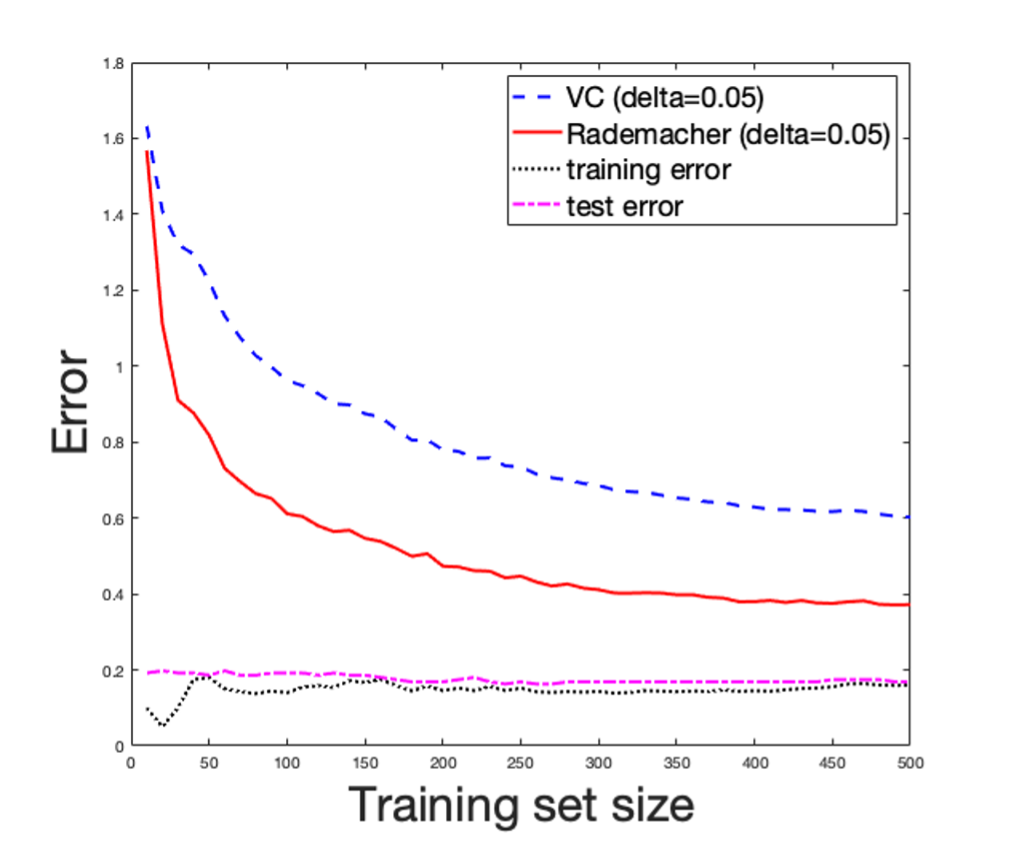
\includegraphics[width=0.7\columnwidth]{images/rademacher-vs-vc.png}
    \caption{Rademacher and VC bounds on a real dataset}
    \label{fig:fig6}
\end{figure}

\begin{itemize}
  \item Rademacher bound is sharper than the VC bound
  \item VC bound is not yet informative with 500 examples $(> 0.5)$ using $(\delta = 0.05)$
  \item The gap between the mean of the error distribution ($\approx$ test error) and the 0.05 probability tail (VC and Rademacher bounds) is evident (and expected)
\end{itemize}



\end{document}
